\documentclass[../../Thesis.tex]{subfiles}

\begin{document}
	
	In this chapter, we will explain the construction process behind the datasets that have been used to train the model and observe the feature's performance. The process is composed of three main steps: running simulations, translating simulation log files into time series, computing robot features time series. The simulations are executed through the simulators introduced in Section \ref{sec:simulators} and will be explained in more detail in Section \ref{sec:running_examples}. The translation of log files into time series data objects is explained in Section \ref{sec:dataset_construction}. Finally, the computation of the features' time series is described in Section \ref{sec:feature_computation}.
	
	\section{Data Retrieval}
		Simulations data is collected through comma separated value files (\verb|.csv|) that are directly written by the simulators. These files are then processed with \verb|python| and all the robots' positions are translated into time-series objects. 
		
		\subsection{Running Examples}
		\label{sec:running_examples} %
			In our experiments, we run several simulations with different settings.  In this section, we will list the settings used for the simulations of each task and show an example of task execution.
			\subsubsection{ARGoS Flocking}
			\label{sec:argos_flocking_simulation_parameters} %
				For the flocking task, we have used a simulation environment of a $30 \times 30$ $m^2$ arena surrounded by walls and with $15$ bots. Even though the walls have never worked as a constraint measure, they are necessary to put physical bounds to the arena. The coordinate system of the simulation is considered to have the $(0,0,0)$ position in the middle of the arena at ground height. The simulations have a duration of $800$ seconds, this value has been chosen arbitrarily after some tests to allow the swarm to complete the task. The goal of the task is to reach a light positioned in the center of the arena at a height of 4 $m$ from the ground, the light coordinates are $(0,0,4)$ and it is oriented toward $(0,0,0)$. The flocking task presumes that the robots manage to reach the light while keeping a formation, more precisely they have to keep a distance of 75 $cm$ from all their neighbors. In our \verb|.argos| settings we specified a \verb|gain| parameter of 1000 for the flocking controller.  The robots begin each flocking simulation from one of the 4 different starting areas, namely North, South, East, and West. We can see the starting positions depicted in Figure \ref{fig:flocking_starting_positions} with their corresponding names and the light in the center of the arena.\\
				Faults have been injected in the 10\%, 20\%, or 33\% of the swarm population and at 0 $s$, 50 $s$, 150 $s$, or 400 $s$ from the beginning of the simulation. Completely nominal simulations are run together with faulty simulations in order to have a complete dataset of a real situation. An example of the robot trajectories can be seen in Figure \ref{fig:ARGoS_flocking_trajectories} where nominal and faulty agents are separated in two different graphs.
				\begin{figure}
				    \centering
				    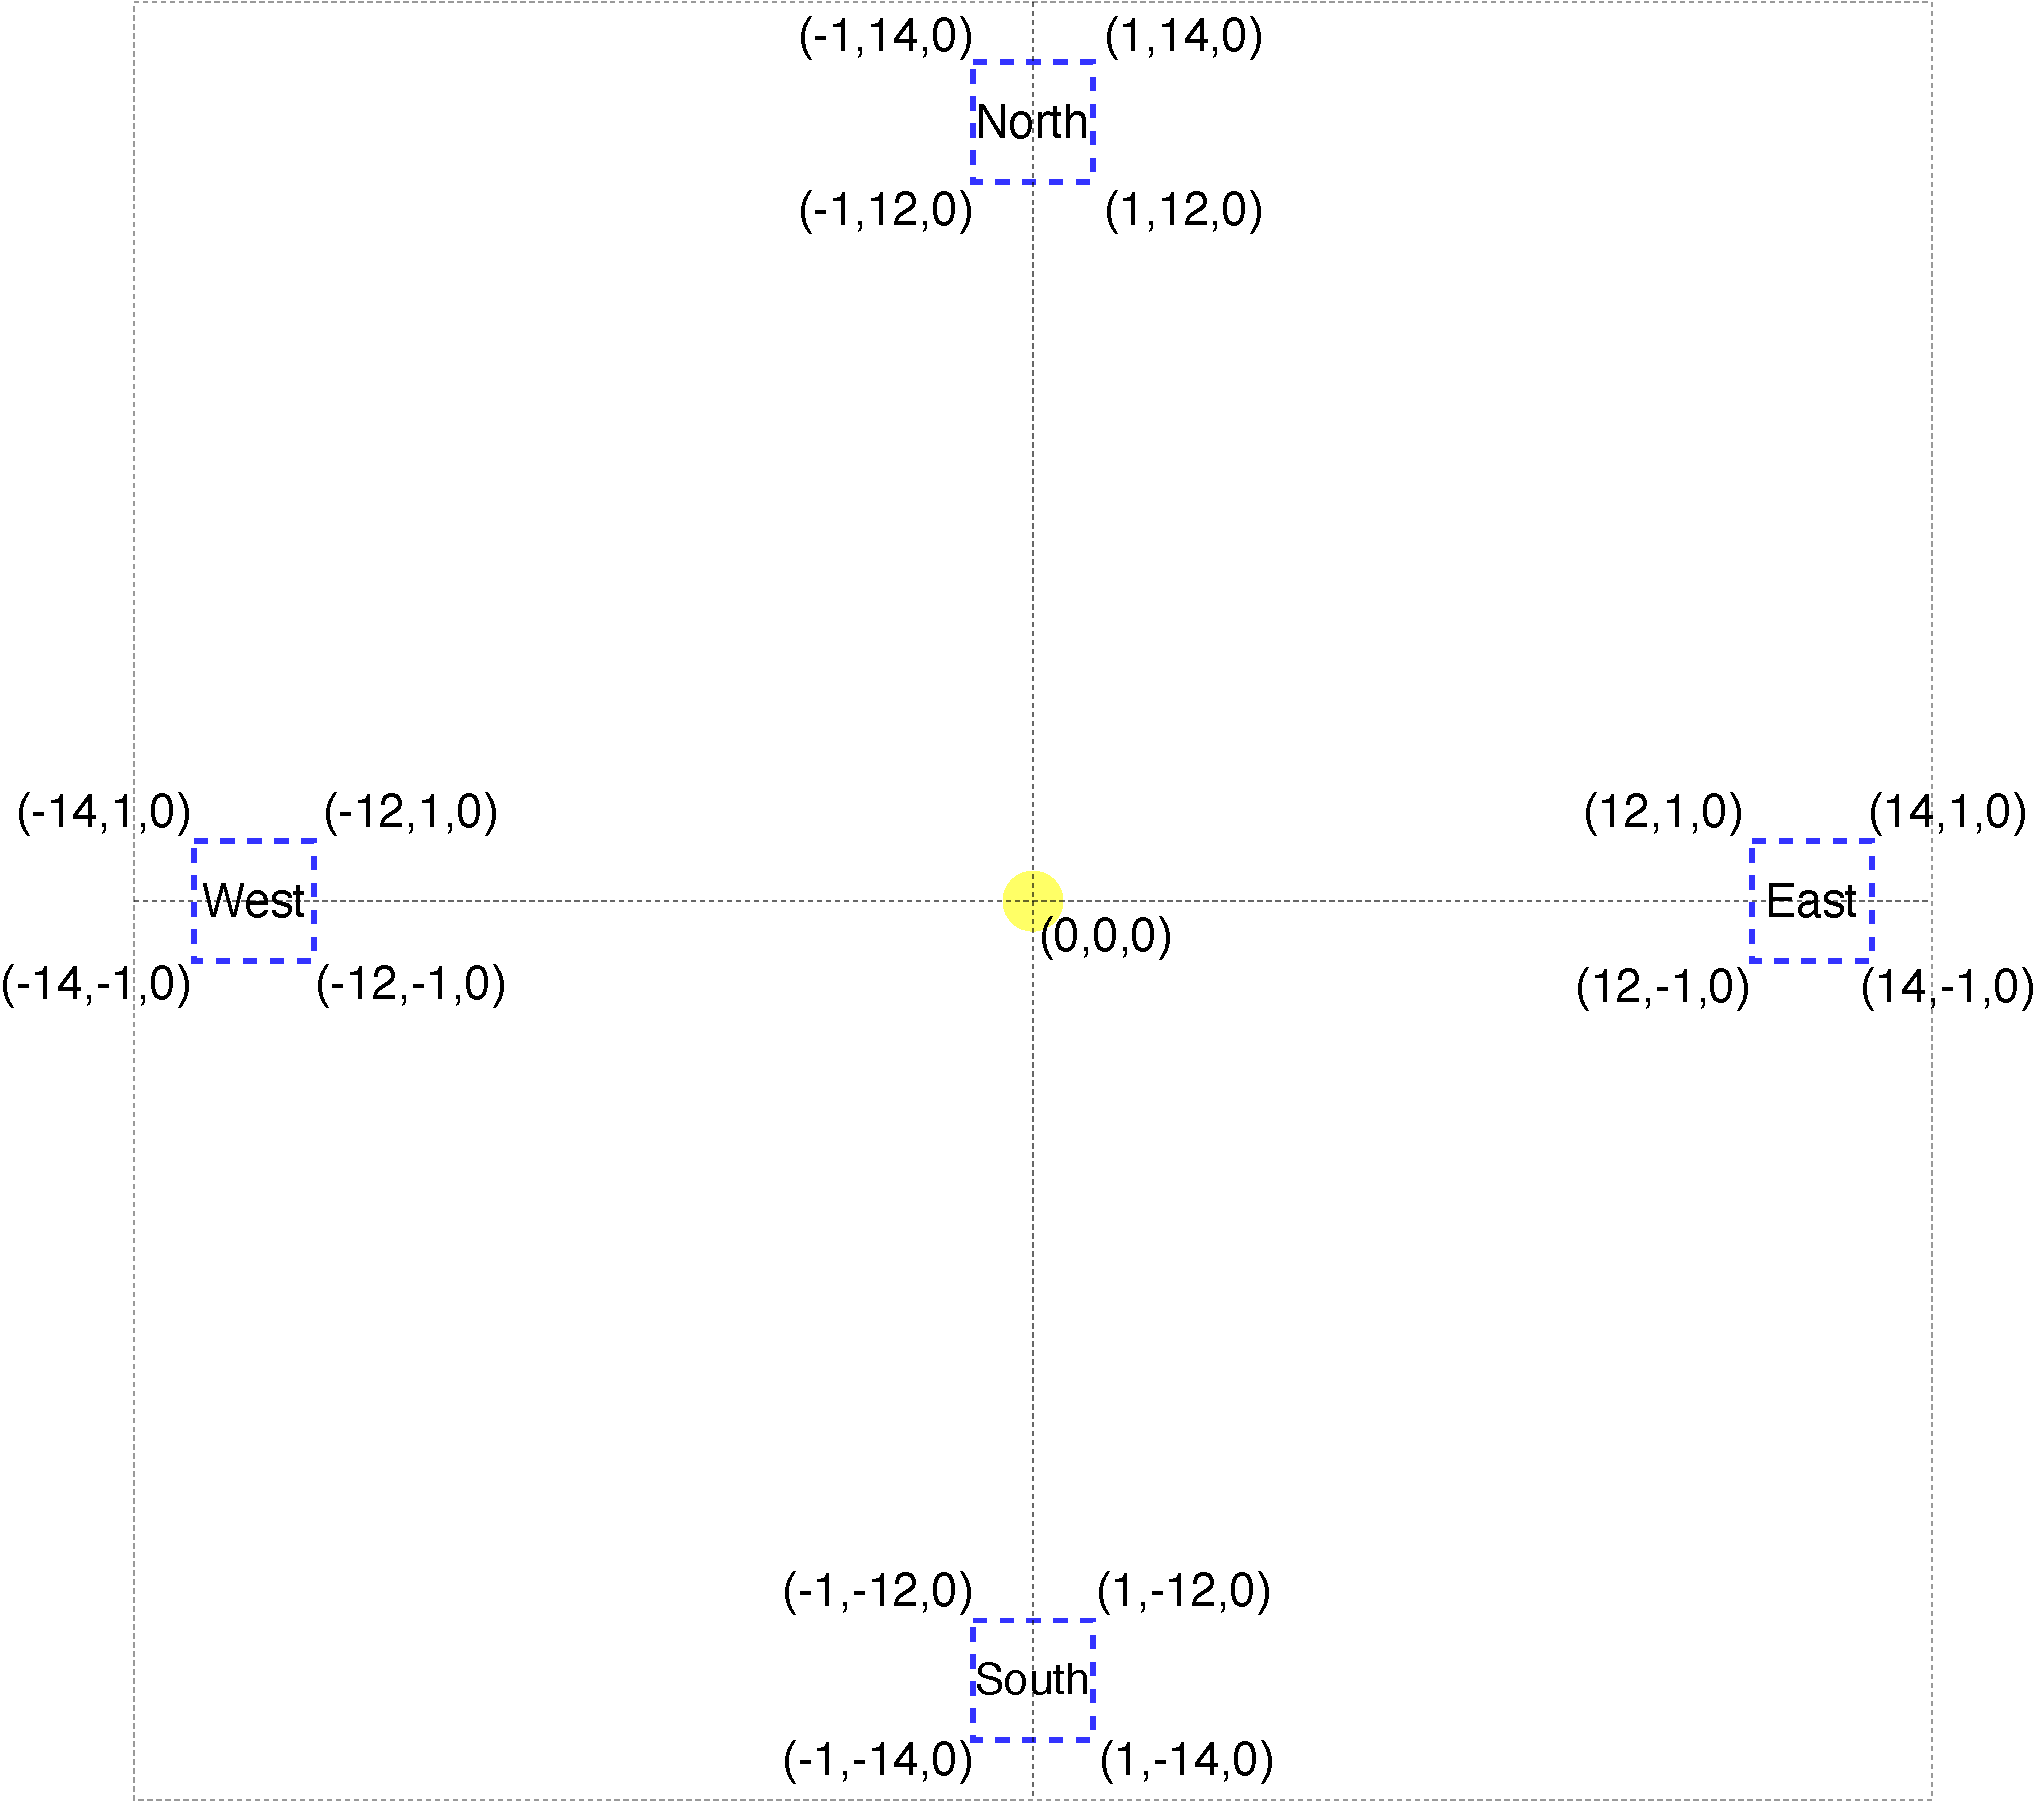
\includegraphics[width=0.8\textwidth]{../../Images/Fault_detection/flocking_coordinates.pdf}
				    \caption{Flocking task robots starting positions.}
				    \label{fig:flocking_starting_positions}
				\end{figure}
				\begin{figure}
				    	\centering
				    	\subfloat[ARGoS flocking nominal bots trajectories.
				    		\label{fig:ARGoS_flocking_nominal_trajectories}]{
				    		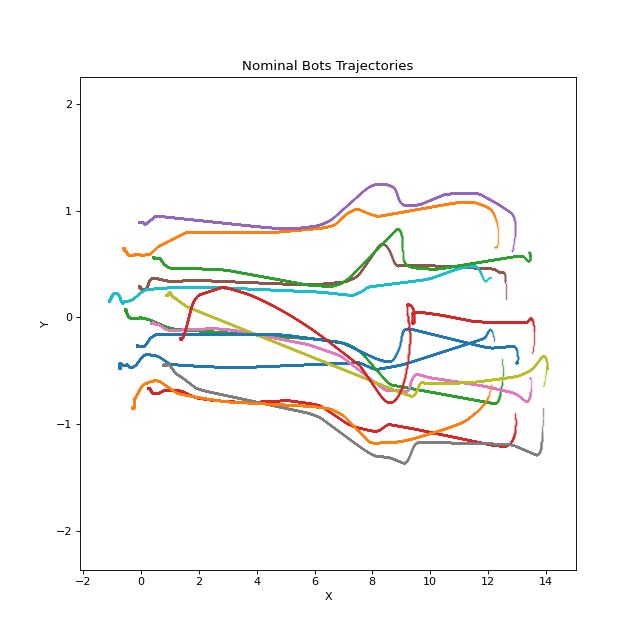
\includegraphics[scale=0.3]{../../Images/Fault_detection/Flocking_Nominal_Bots_Trajectories.png}
				    }
				    \quad
				    \subfloat[ARGoS flocking faulty bots trajectories.\label{fig:ARGoS_flocking_fault_trajectories}]{
				        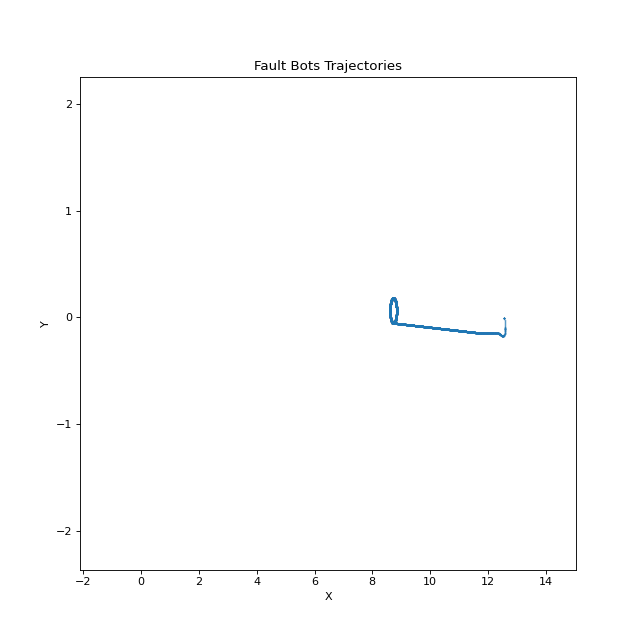
\includegraphics[scale=0.3]{../../Images/Fault_detection/Flocking_Fault_Bots_Trajectories.png}
				    }
				    \caption{ARGoS flocking plotted trajectories.}
				    \label{fig:ARGoS_flocking_trajectories}
				\end{figure}
				
			\subsubsection{ARGoS Foraging}
			\label{sec:argos_foraging_simulation_parameters} %
				For the foraging task, we have used incremental settings that adapts with the increase of the arena size. The arena size starts from $5\times5$ $m^2$ and ends in $8 \times 8$ $m^2$ going trough each possible combination with sides of size $\lbrace 5, 6, 7, 8 \rbrace$ $m$ thus using 16 different arena sizes. In this task, the arena is surrounded by walls and they're fundamental to keep the bot inside the arena while they're performing the random walk. The goal of the task is to retrieve the items in the resource area and bring them to the nest area. There are 4 lights to signal the position of the nest on the nest side of the arena, they're positioned at a height of 1 $m$ from the ground. The lights' coordinates change with the size of the arena. At each simulation, they are positioned at the 10\%, 30\%, 70\%, and 90\% of the wall length in order to be adequately distanced. The robot number starts from 20 agents and scales in a directly proportional way with the arena size. The simulations last 800 seconds, this value has been chosen arbitrarily but the task execution does not depend on it as it is for flocking. The foraging task requires some parameters for the agents' foraging behavior, these values are scaled with the arena size in order to have coherent simulations among different arenas. The foraging task parameters are: 
				\begin{itemize}
					\item \verb|minimum_resting_time| parameter: initialized at 5 $s$.
					\item \verb|minimum_unsuccessful_explore_time| parameter: initialized at 60 $s$.
					\item \verb|minimum_search_for_place_in_nest_time| parameter: is initialized at 15 $s$.
				\end{itemize}
				Each foraging simulation requires a number of items to be scattered around in the resources area, this value is initialized at 15 items and scales with the arena size. An example of the foraging arena can be seen in Figure \ref{fig:foraging_arena_graph}. \\
				For each arena size, a number of nominal simulations are executed together with a number of simulations with injected faults. For the faulty simulations, we have considered 10\%, 20\%, or 33\% of the swarm population to be infected at 0, 100, or 400 $s$ from the task start.  An example of the robot trajectories can be seen in Figure \ref{fig:ARGoS_foraging_trajectories} where nominal and faulty agents are separated in two different graphs.
				\begin{figure}
				    \centering
				    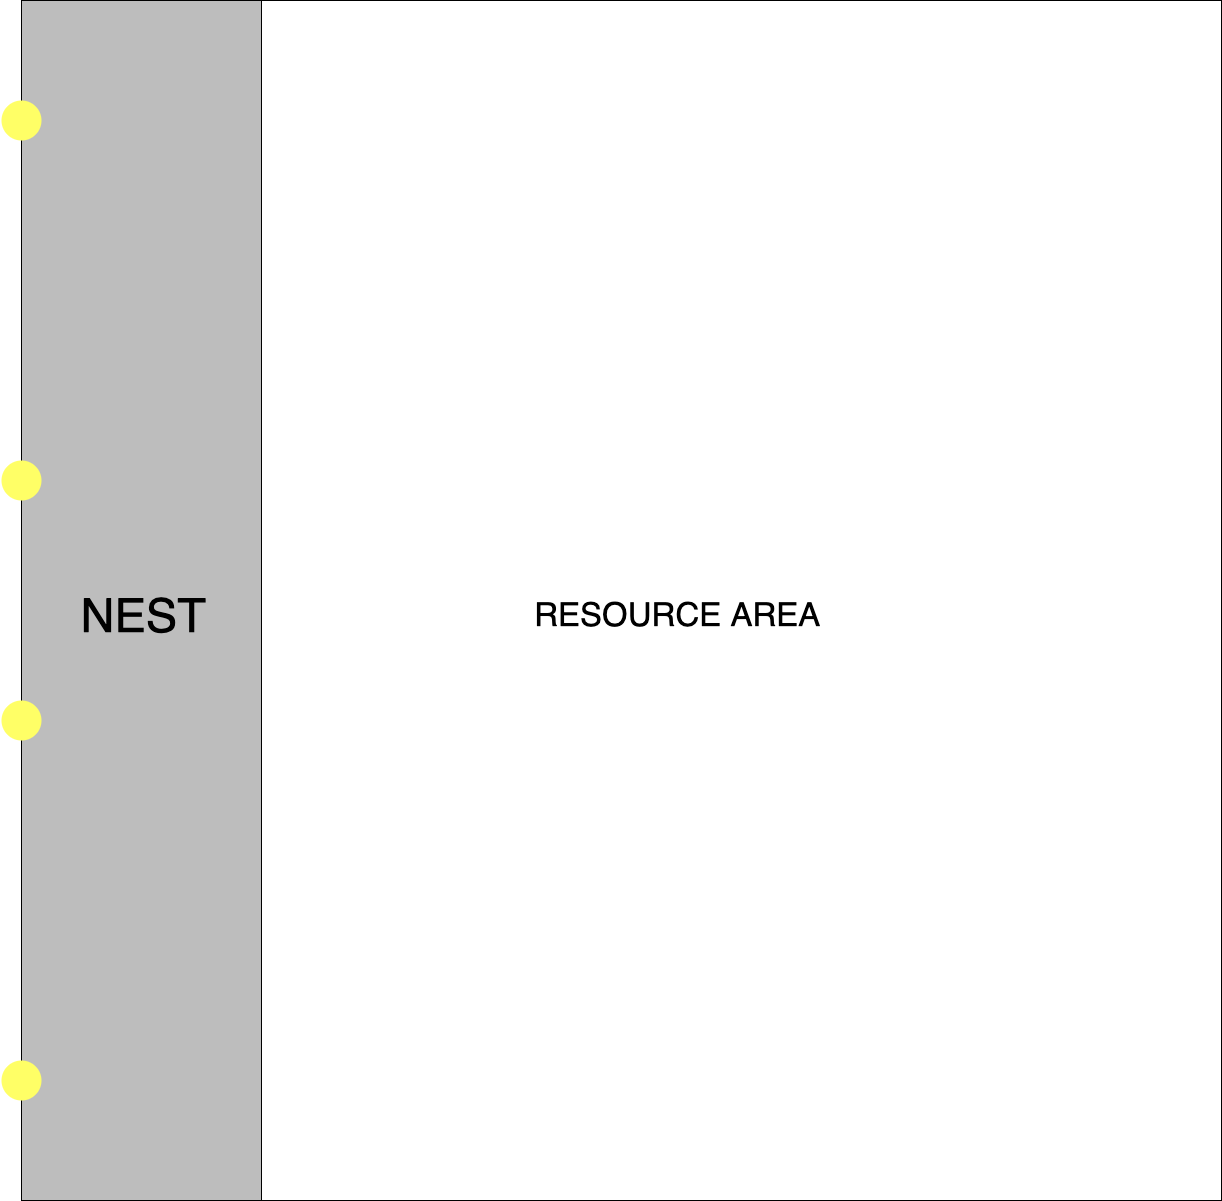
\includegraphics[width=0.6\textwidth]{../../Images/Fault_detection/foraging_arena.png}
				    \caption{Foraging arena example.}
				    \label{fig:foraging_arena_graph}
				\end{figure}
				\begin{figure}
				    	\centering
				    	\subfloat[ARGoS foraging nominal bots trajectories.
				    		\label{fig:ARGoS_foraging_nominal_trajectories}]{
				    		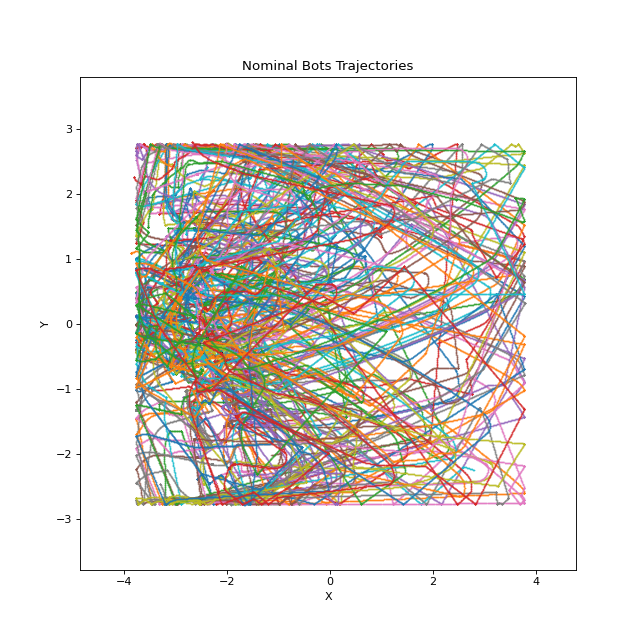
\includegraphics[scale=0.3]{../../Images/Fault_detection/Foraging_Nominal_Bots_Trajectories.png}
				    }
				    \quad
				    \subfloat[ARGoS foraging faulty bots trajectories.\label{fig:ARGoS_foraging_fault_trajectories}]{
				        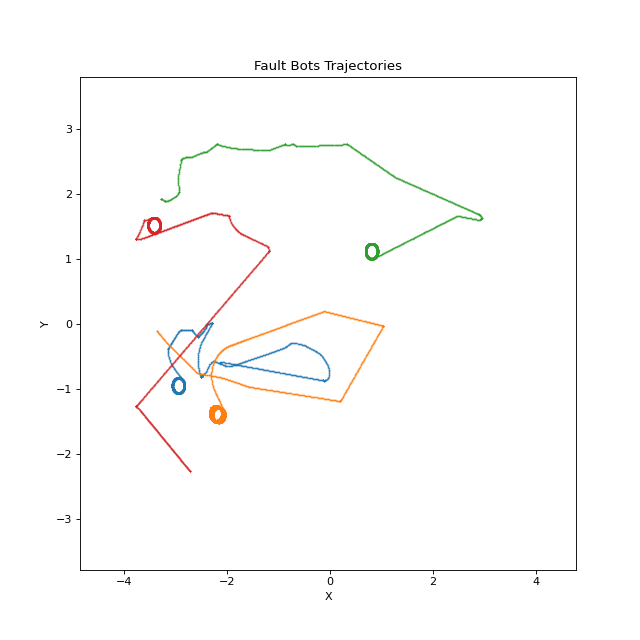
\includegraphics[scale=0.3]{../../Images/Fault_detection/Foraging_Fault_Bots_Trajectories.png}
				    }
				    \caption{ARGoS foraging plotted trajectories.}
				    \label{fig:ARGoS_foraging_trajectories}
				\end{figure}
				
			\subsubsection{RAWSim-O Fulfillment System}
			\label{sec:fault_detection:RAWSim-O_fulfillment_system}%
				The RMFS task is set in a warehouse sized by the number of horizontal and vertical aisles that the robots use to move. In our experiments we used different arena sizes starting from $5 \times 5$ horizontal aisles $\times$ vertical aisles size through $8 \times 8$ horizontal aisles $\times$ vertical aisles, using each combination of the aisles number in $\lbrace 5, 6, 7, 8 \rbrace$, thus 16 different warehouse sizes. The environment objects are placed by the simulators, between each aisle there is a group of 10 pods locations that do not have to be all occupied.  The simulations have a duration of 80000 seconds which approximately simulates the duration of a workday.  The goal of the task is to follow the orders of the RMFS and carry pods from the storage area to the pick stations and replenishment stations.  Based on how many horizontal aisles are included in the warehouse there is a corresponding number of pick stations and replenishment stations, the rule the compute the stations' number is:
				\[\text{stations number} = \lfloor \frac{\text{horizontal aisles number}}{2} \rfloor .\]
				The robot number starts from 15 agents and scales in a directly proportional way with the arena size.  We can see an example of the warehouse environment in Figure \ref{fig:rawsim_o_2d}. \\
				For each warehouse size, a number of nominal simulations have been executed together with a number of simulations with injected faults. For the faulty simulations, we have considered 5\%,10\%, 20\%, or 33\% of the swarm population to be infected from the start of the task with a reduced speed of 10\% or 5\% of the maximum speed.  An example of the robot trajectories can be seen in Figure \ref{fig:RAWSim-O_trajectories} where nominal and faulty agents are separated in two different graphs.
				\begin{figure}
				    \centering
				    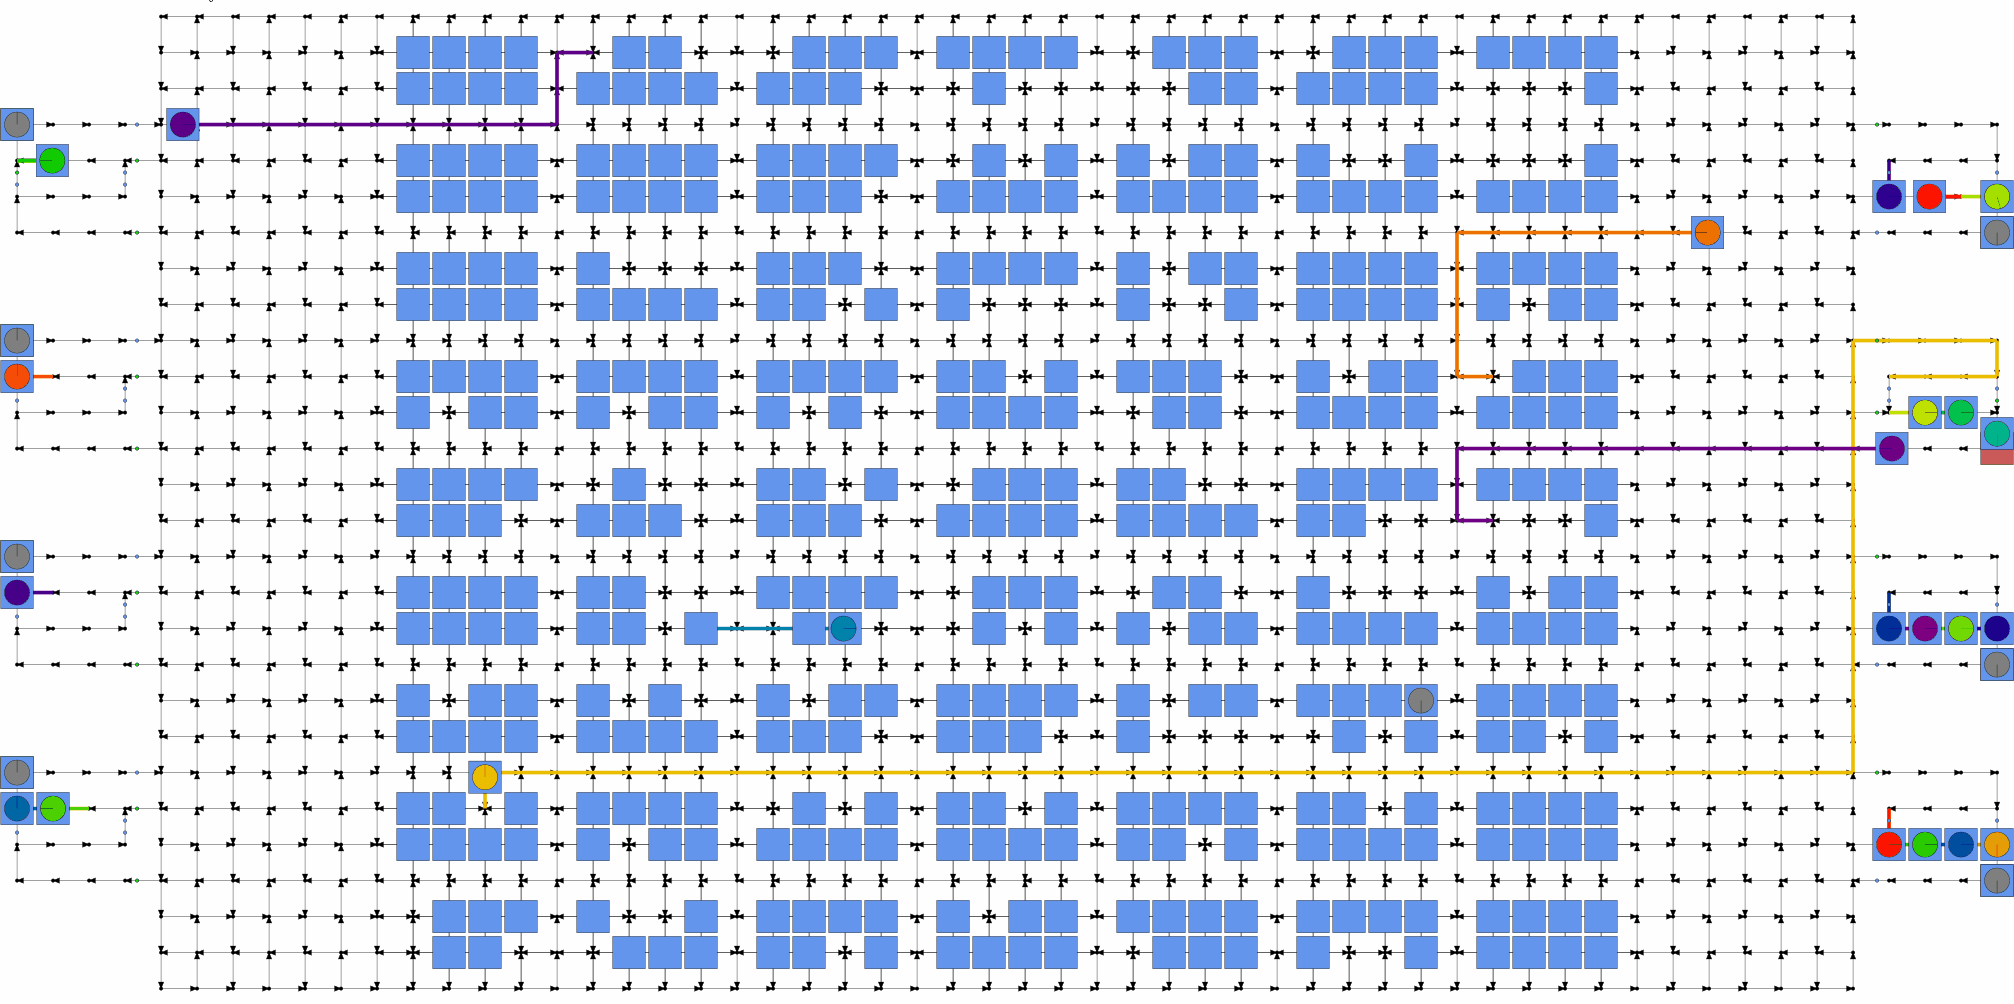
\includegraphics[width=0.6\textwidth]{../../Images/Fault_detection/rawsim-o-2d.png}
				    \caption{RMFS warehouse example.}
				    \label{fig:rawsim_o_2d}
				\end{figure}
	 			\begin{figure}
				    	\centering
				    	\subfloat[RAWSim-O nominal bots trajectories.
				    		\label{fig:RAWSim-O_nominal_trajectories}]{
				    		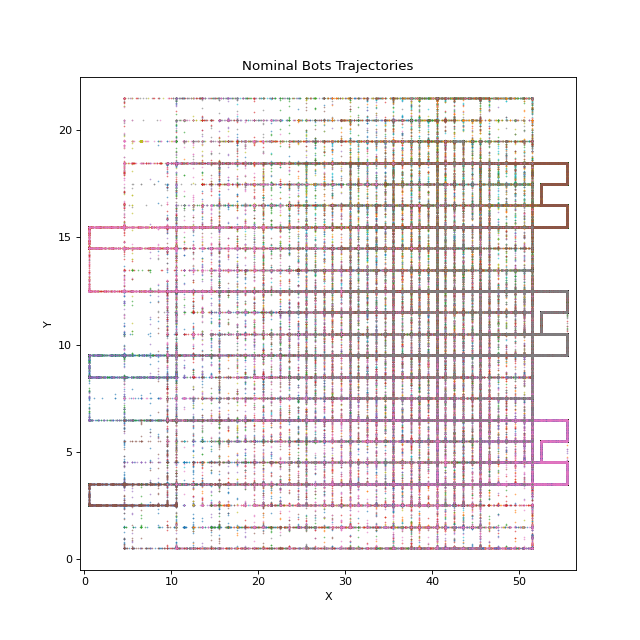
\includegraphics[scale=0.3]{../../Images/Fault_detection/Warehouse_Nominal_Bots_Trajectories.png}
				    }
				    \quad
				    \subfloat[RAWSim-O faulty bots trajectories.\label{fig:RAWSim-O_fault_trajectories}]{
				        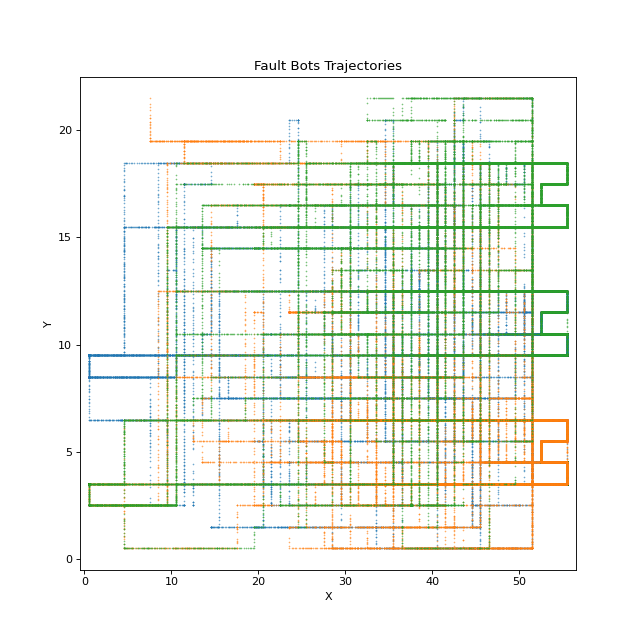
\includegraphics[scale=0.3]{../../Images/Fault_detection/Warehouse_Fault_Bots_Trajectories.png}
				    }
				    \caption{RAWSim-O plotted trajectories.}
				    \label{fig:RAWSim-O_trajectories}
				\end{figure}
				
	\section{Simulation Data Translation}
	\label{sec:dataset_construction} %
		During each simulation, the simulator is responsible for writing a \verb|.csv| file where the information of every bot at every timestep is written. At the end of the simulation, we are provided with a \verb|.csv| file with a structure identical to that of Table \ref{tab:csv_file_structure} but filled with values for each timestep and robot identification code. This step is supposed to simulate the external controller that observes the execution of the task and identifies each agent's position. The Fault value is necessary to perform supervised learning, in real-world scenarios it will not be provided.
		\begin{table}[H]
		\centering 
		    \begin{tabular}{| c | c | c | c | c |}
			    \hline
				\rowcolor{bluepoli!40}
				\textbf{timestep} & \textbf{ID} & \textbf{PosX} & \textbf{PosY} & \textbf{Fault} \T\B \\
			    \hline \hline
			    1 & 0 & 12.5606 & -0.0025857 & 0 \T\B\\
			    1 & 1 & 12.2117 & -0.222327 & 0 \T\B\\
			    $\dots$ & $\dots$ & $\dots$ & $\dots$ & $\dots$ \T\B\\
			    1501 & 0 & 8.72475 & -0.0530649 & 1 \T\B\\
			    $\dots$ & $\dots$ & $\dots$ & $\dots$ & $\dots$ \T\B\\
			    8000 & 0 & 8.66732 & -0.0364418 & 1 \T\B\\
			    $\dots$ & $\dots$ & $\dots$ & $\dots$ & $\dots$ \T\B\\
			    8000 & 14 & -0.0665298 & 0.290923 & 0 \T\B\\
			    \hline
		    \end{tabular}
		    \\[10pt]
		    \caption{Comma separated values file structure.}
		    \label{tab:csv_file_structure}
		\end{table}
		
 	\section{Feature Computation}
 	\label{sec:feature_computation} %
		The feature list has is shown in Table \ref{tab:feature_list}. In this section we will explain how each feature has been computed.
	 		\bgroup
	 		\def\arraystretch{1.5}
	 		\begin{table}
		 		\begin{tabular}{|l|l|}
		 			\hline
		 			\rowcolor{bluepoli!40}
		 			\hline
		 			\multicolumn{1}{|c|}{\textbf{Feature}} & \multicolumn{1}{|c|}{\textbf{Description}} \T\B \\
		 			\hline
		 			Position & Coordinates of the agent in a single timestep \\
		 			Direction & Directional vectors on x and y axis \\
		 			Speed & Velocity of the agent between two consecutive timesteps\\
		 			Cumulative speed & Sum of the last $n$ timesteps velocity values\\
		 			Neighbors number & Number of agent within a specified radius\\
		 			Neighbors average distance & Average distance from all the bots in the swarm\\
		 			Centroid distance & Distance from the coordinates of the swarm centroid\\
		 			Cumulative centroid distance & Sum of the last $n$ centroid distance values\\
		 			Position entropy & Entropy measure of the last $n$ positions\\
		 			Area coverage & Percentage of area covered by the agent\\
		 			Speed area coverage & Area coverage between two consecutive timesteps\\
		 			Swarm position & Coordinates of the swarm centroid\\
		 			Swarm speed & Velocity of the centroid between two consecutive timestep\\
		 			Swarm area coverage & Percentage of area covered by the whole swarm\\
		 			\hline
		 		\end{tabular}
		 		\caption{Single bot list of features.}
		 		\label{tab:feature_list}
	 		\end{table}
	 		\egroup
	 	
		\subsection{Position, Direction, Speed, Cumulative Speed}
			The position feature is the transposition of the \verb|PosX| and \verb|PosY| values into a \verb|numpy| vector of size $[\text{timestep number}, 2]$. For future references, we will refer to this feature as $pos_{x,i}$ where $x$ represents the x-axis and $i \in [0, \dots, T]$ is the timestep in a simulation of length $T$.\\
			The direction feature is computed by subtracting the current position value from the previous position value for the x-axis and y-axis:
			\[dir_{x,i} = pos_{x,i-1} - pos_{x,i}.\]
			The speed feature is computed as the rate of change of position with respect to time:
			\begin{equation}
				v_i = 
				\frac{\sqrt{(pos_{x,i-1} - pos_{x,i})^2 + (pos_{y,i-1} - pos_{y,i})^2}}
					{t_{i} - t_{i-1}}
				\label{eq:speed_computation}
			\end{equation}
			with $v_0 = 0 \frac{m}{s}$.\\
			The cumulative speed feature for agent $i$ at timestep $t$ is computed as:
			\[\text{cum-}v_{i,t} = 
					\sum\limits_{j=t-(\texttt{time-window})}^T v_{i,j}
			\]
		
		\subsection{Neighbors Number, Neighbors Average Distance}
			The neighbors number feature holds the information about how many other agent are within a predefined radius $r$. It is computed with the Algorithm \ref{alg:neighbor_number} with $N$ as the swarm cardinality, $T$ as the total number of timestep.
			\begin{algorithm}
	 		 	\caption{Neighbors Number Computation.}
	 		 	\label{alg:neighbor_number}
			    	\begin{algorithmic}[1]
			    	\FOR{$t=1$ to $T$}
			    		\STATE{temp-number=0}
			    		\FOR{$i=1$ to $N$}
				    		\STATE{Compute $d$=distance between current agent and agent$_i$.}
				    		\IF{$d<r$}
				    			\STATE{temp-number+=1}
				    		\ENDIF
				    	\ENDFOR
			    		\STATE{neighbors-number$_t$=temp-number}
			    	\ENDFOR
			    	\end{algorithmic}
			\end{algorithm}
			The neighbors average distance feature is computed as the mean value among the distance from the current agent and all the other agents. It is computed with the Algorithm \ref{alg:neighbor_average_distance} with $N$ as the swarm cardinality, $T$ as the total number of timestep.
			\begin{algorithm}
	 		 	\caption{Neighbors Average Distance Computation.}
	 		 	\label{alg:neighbor_average_distance}
			    	\begin{algorithmic}[1]
			    	\FOR{$t=1$ to $T$}
			    		\STATE{distances=$\lbrace \rbrace$.}
			    		\FOR{$i=1$ to $N$}
				    		\STATE{Compute $d$=distance between current agent and agent$_i$.}
				    		\STATE{Add $d$ to distances.}
				    	\ENDFOR
			    		\STATE{avg-$d_t = \frac{\sum_{d \in \text{distances}} d}{N}$}
			    	\ENDFOR
			    	\end{algorithmic}
			\end{algorithm}
		
		\subsection{Position Entropy}
			The position entropy feature computes the entropy of the positions in the last \verb|time-window|$\times 10$ timesteps.  The entropy is computed with \verb|scipy.stats.entropy| \cite{SciPy} module that uses the following formula:	
			\[S = -\sum\limits_{v \in Values}(P(v) * log(P(v)))\]
			The entropy computation procedure is stated in Algorithm \ref{alg:position_entropy}.
			\begin{algorithm}
	 		 	\caption{Position Entropy Computation.}
	 		 	\label{alg:position_entropy}
			    	\begin{algorithmic}[1]
			    	\FOR{$t=1$ to $T$}
			    		\IF{$t<\texttt{time-window}$}
			    			\STATE{Compute vector of probabilities $P$ for each in position in the last $t$ positions.}
			    			\STATE{$entropy_t = -\sum\limits_{p \in P}(p * log(p))$}
			    		\ELSE
			    			\STATE{Compute vector of probabilities $P$ for each in position in the last \verb|time-window| positions.}
			    			\STATE{$entropy_t = -\sum\limits_{p \in P}(p * log(p))$}
			    		\ENDIF
			    	\ENDFOR
			    	\end{algorithmic}
			\end{algorithm}
		
		\subsection{Centroid Distance,Cumulative Centroid Distance}
			The centroid distance feature is the distance of the current agent from the centroid of the swarm. The centroid of the swarm is computed as the mean of the position of all the agents.  Once the swarm centroid time series has been computed, each agent computes the distance between its current position and the position of the swarm centroid. The procedure is shown in Algorithm \ref{alg:centroid_distance_computation}.
			\begin{algorithm}
	 		 	\caption{Centroid Distance Computation.}
	 		 	\label{alg:centroid_distance_computation}
			    	\begin{algorithmic}[1]
				    	\FOR{$t=1$ to $T$}
				    		\STATE{$centroid\text{-}pos_t = \frac{\sum\limits_{i \in N} pos_i}{|N|}$}
				    	\ENDFOR
				    	\FOR{$i=1$ to $N$}
				    		\FOR{$t=1$ to $T$}
				    			\STATE{$centroid\text{-}distance_{i,t} = centroid\text{-}pos_t - pos_{i,t}$}
				    		\ENDFOR
				    	\ENDFOR
			    	\end{algorithmic}
			\end{algorithm}
			The cumulative centroid distance feature for agent $i$ at timestep $t$ is computed as:
			\[\text{cum-}centroid\text{-}distance_{i,t} = 
					\sum\limits_{j=t-(\texttt{time-window})}^t centroid\text{-}distance_{i,j}
			\]
		
		\subsection{Area Coverage, Speed Area Coverage}
		\label{sec:Fault_detection:area_coverage_speed_area_coverage}%
			The area coverage feature represents the area percentage covered by the agent until that exact moment.  It is computed with 4 different levels of detail: 4, 16, 64, and 256 subdivision of the total area available. Area subdivisions are computed with the maximum and minimum positions covered by any robot in each axis. An approximate algorithm of the procedure is shown in Algorithm \ref{alg:area_bounds}, the real implementation is optimized using \verb|numpy| array and python functional programming with list comprehension.\\
			Once the area borders have been computed, these values are used to compute the area coverage percentage of each agent. The area coverage computation procedure is shown in Algorithm \ref{alg:area_coverage}.\\
			The area coverage speed feature holds the information about the value increment in the area coverage timeseries for each timestep. The procedure to compute the area coverage speed feature is shown in Algorithm \ref{alg:area_coverage_speed}.
			\begin{algorithm}
	 		 	\caption{Area bounds computation.}
	 		 	\label{alg:area_bounds}
			    	\begin{algorithmic}[1]
				    	\STATE{Initialize variables to store positions. In this algorithm we will consider the order (agent-id, timestep-number,coordinate-axis) for the subscripts of $pos$}
			    		\STATE{min-pos-x = $pos_{1,1,x}$}
			    		\STATE{min-pos-x = $pos_{1,1,y}$}
			    		\STATE{max-pos-x = $pos_{1,1,x}$}
			    		\STATE{max-pos-x = $pos_{1,1,y}$}
				    	\FOR{$i=1$ to $N$}
				    		\FOR{$t=1$ to $T$}
				    			\IF{min-pos-x $> pos_{i,t,x}$}
				    				\STATE{min-pos-x = $pos_{i,t,x}$}
				    			\ENDIF
				    			\IF{min-pos-y $> pos_{i,t,y}$}
				    				\STATE{min-pos-y = $pos_{i,t,y}$}
				    			\ENDIF
				    			\IF{max-pos-x $< pos_{i,t,x}$}
				    				\STATE{max-pos-x = $pos_{i,t,x}$}
				    			\ENDIF
				    			\IF{max-pos-y $< pos_{i,t,y}$}
				    				\STATE{max-pos-y = $pos_{i,t,y}$}
				    			\ENDIF
				    		\ENDFOR
				    	\ENDFOR
				    	\FOR{$split \in \lbrace 2,4,8,16 \rbrace $}
				    		\FOR{$i=1$ to $split$}
				    			\STATE{Compute segment$_{x,i}$ coordinates from the subdivision of segment $\left[ \text{min-pos-x}, \text{max-pos-x} \right]$ in equal $split$ parts}
				    			\STATE{Compute segment$_{y,i}$ coordinates from the subdivision of segment $\left[ \text{min-pos-y}, \text{max-pos-y} \right]$ in equal $split$ parts}
				    			\STATE{Save segments coordinates in an AreaPartition object.}
				    			\STATE{Save AreaPartition object in the area-subdivision list.}
				    		\ENDFOR
				    		\STATE{Save area-subdivision list object in the area-partitions list.}
				    	\ENDFOR
			    	\end{algorithmic}
			\end{algorithm}
			
			\begin{algorithm}
	 		 	\caption{Area coverage computation.}
	 		 	\label{alg:area_coverage}
			    	\begin{algorithmic}[1]
			    		\STATE{Consider current agent $i$.}
				    	\FOR{area-subdivisions list in area-partitions list}
				    		\STATE{timestep=0.}
			    			\WHILE{any AreaPartition not visited \& timestep $< T$}
			    				\FOR{area-partition in not visited area-partitions}
			    					\IF{$pos_{i,t}$ is in area-partition}
				    					\STATE{area-partition.visited=True.}
				    				\ENDIF
			    				\ENDFOR
			    				\STATE{area-coverage$_{i,t} = 
			    					\frac{\sum\limits_{\text{area} \in \text{area-partitions-list}} I(\text{area.visited()==True)}}{|\text{area-partitions-list}|}$ }
			    				\STATE{timestep+=1.}
			    			\ENDWHILE
			    			\IF{iteration ends before visiting all timesteps}
			    				\STATE{fill area-coverage$_i$ timeseries with the last computed value.}
			    			\ENDIF
				    	\ENDFOR
			    	\end{algorithmic}
			\end{algorithm}
			
			\begin{algorithm}
	 		 	\caption{Area coverage speed computation.}
	 		 	\label{alg:area_coverage_speed}
			    	\begin{algorithmic}[1]
			    		\STATE{Consider current agent $i$.}
				    	\FOR{$t=1$ to $T$}
				    		\STATE{coverage-speed$_i$ = area-coverage$_{i,t}$ - area-coverage$_{i,t-1}$}
				    	\ENDFOR
				    	\STATE{Repeat for each area-subdivision level.}
			    	\end{algorithmic}
			\end{algorithm}
			
		\subsection{Swarm Position, Swarm Speed, Swarm Area Coverage}
			The swarm position feature represents the coordinates of the entire swarm, for this feature we've used the centroid of the positions of all the robots. The swarm position computation can be seen from line 1 to line 3 of Algorithm \ref{alg:centroid_distance_computation}.\\
			The swarm speed is computed as the speed feature for the single agent, in fact, we can refer to Equation \ref{eq:speed_computation} to compute the swarm speed considering the swarm centroid instead of the single agent position.\\
			The swarm area coverage is considered as an overall area coverage performed by the whole swarm. The computation of the swarm area coverage feature is similar to the one shown in Algorithm \ref{alg:area_bounds} and Algorithm \ref{alg:area_coverage} with the only difference that, when we check if an area partition is visited, we check if any robot in the whole swarm is covering that area. 
	 	
\end{document}
